\documentclass[/Users/ikedahajime/GitHub/reserch/master_report/thesis]{subfiles}
% このファイル内だけのコマンド
\begin{document}
% \chapter{壁の形状による影響}\label{subsec:result_abp_twowall}
% 2つの円を繋げて、それらの円における渦が同じ方向に回る(強磁性的)か反対の方向に回る(反強磁性的)か
% を調べた研究が存在する\cite{beppuGeometrydrivenCollectiveOrdering2017}。この研究では、強磁性、反強磁性を
% 分ける要素は2つの円の間の距離であることがわかっている。この章では自己駆動力がこの現象に与える
% 影響を明らかにするため、ABPについてのシミュレーションを行う。%TODO:言い回し
\section{壁の形状による影響}\label{sec:res_abp_twowall}
\subsubsection{低密度系}
\subsubsection{高密度系}


その結果は\figref{fig:twocer_lo0.7_r10_m0.1}の通りである。
半径$R=10$、$\varphi=0.7、M=0.1$のパラメータを用いた。

\begin{figure}
    \centering
    \begin{tabular}{c}
        \begin{minipage}{0.4\hsize}
            \text{(a)}
            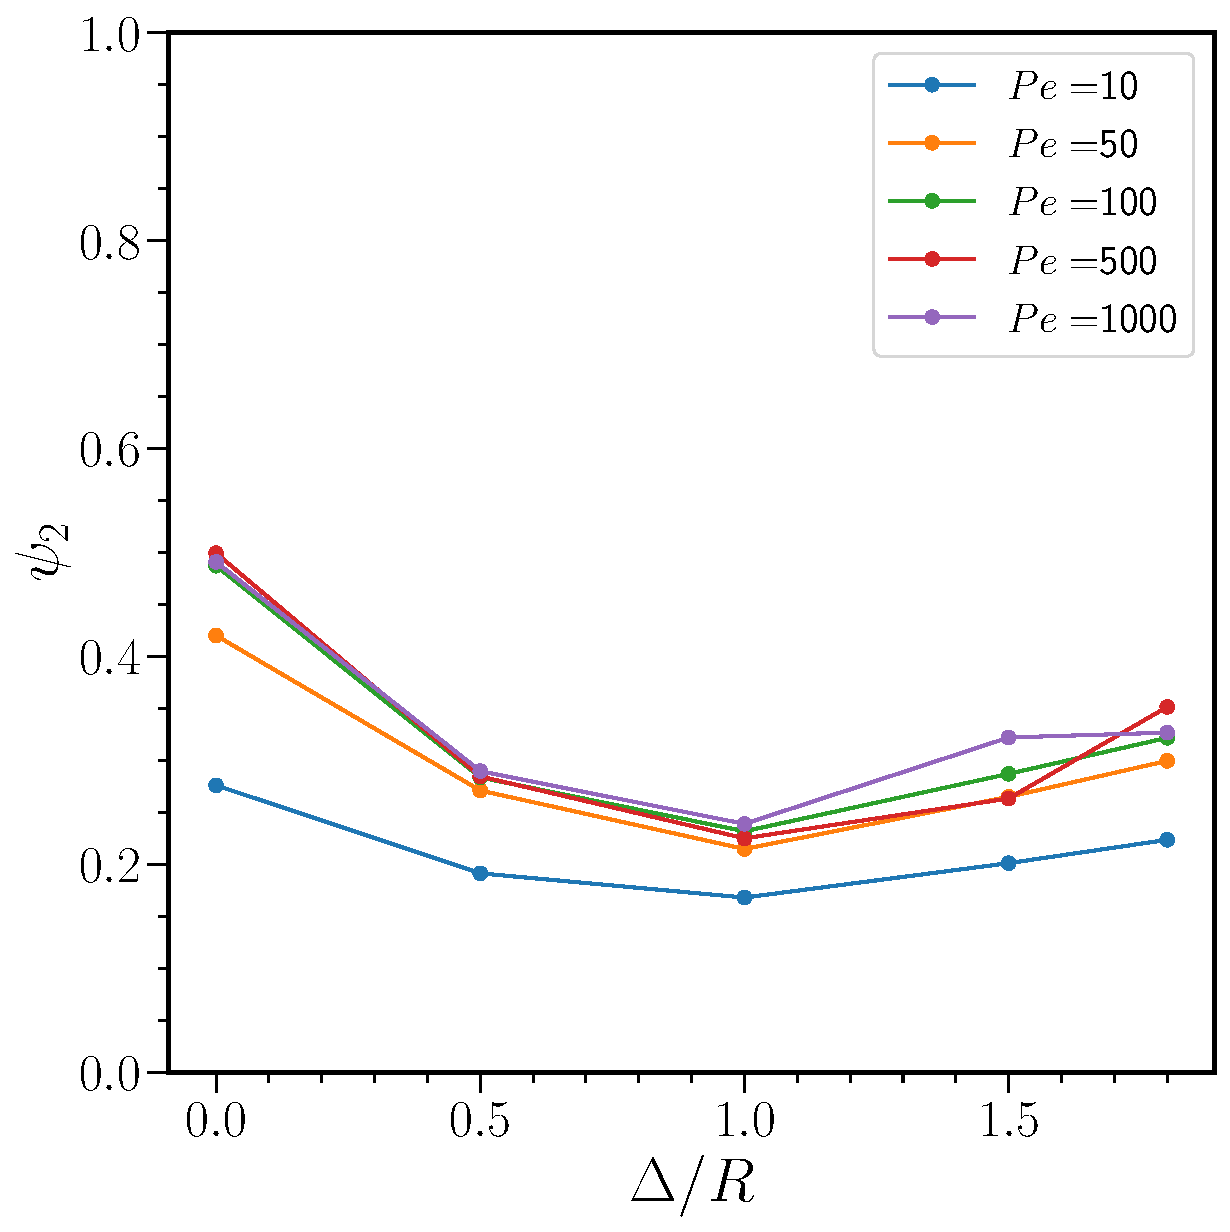
\includegraphics[width=\textwidth]{img/bit/ani_test/psi_20.70.110.pdf}
        \end{minipage}
        % \begin{minipage}{0.3\hsize}
        %     \text{(b)}
        %     \includegraphics[width=\textwidth]{img/bit/ani_test/L_{z2}0.70.110.pdf}
        % \end{minipage}
        \begin{minipage}{0.4\hsize}
            \text{(b)}
            \includegraphics[width=\textwidth]{img/bit/ani_test/V_{2}0.70.110.pdf}
        \end{minipage}
    \end{tabular}
    \caption[two_hdlm]
    {
        $\varphi=0.7、R=10、M=0.1$における(a)$\varphi_2$、(b)$V_2$のグラフ。
        横軸は2つの円の間の距離である。
    }
    \label{fig:twocer_lo0.7_r10_m0.1}
\end{figure}
まず$Pe$依存性について見ると、$\varphi_2、V_2$においてそれらの絶対値が大きくなっており、円が1つの場合
と同様に$Pe$が大きくなると粒子が同じ方向へと流れることがわかる。
次に$\Delta$依存性について見ると、$\Delta\simeq1.4$周りで$V_2$の符号が正から負へと変化しており、
これは$\Delta$を大きくすると2つの円の流れが同じ方向から逆の流れへと変化することを表す。
\end{document}

